\documentclass[12pt]{article}

\usepackage{xspace}
\usepackage{lineno}
\usepackage{setspace}
\usepackage{graphicx}
\usepackage{subfigure}
\usepackage{float}
\usepackage{color}
\usepackage{caption}
\usepackage[margin=1in]{geometry}
\usepackage{epstopdf}
\usepackage{natbib}

\begin{document}
\doublespacing
\linenumbers

\newcommand{\kluyveri}{\textit{L. kluyveri}\xspace}


\noindent RH: LANDERER ET AL.--- Intragenomic variation in codon usage
% put in your own RH (running head)
% for POVs the RH is always POINT OF VIEW
\bigskip
\medskip
\begin{center}

% Insert your title:
\noindent{\Large \bf Differences in Codon Usage Bias between genomic regions in the yeast \textit{Lachancea kluyveri}.}
\bigskip

% We don't use a special title page; the author information is entered
% like any other text.

% FOOTNOTES: We don't allow them in the manuscript, except in
% tables. Don't include any footnotes in the text.


\noindent{C\textsc{EDRIC} ~{L\textsc{ANDERER}}$^{1,2,*}$,
R\textsc{USSELL} {Z\textsc{ARETZKI}}$^{3}$,
\textsc{AND}
M\textsc{ICHAEL} A.~{G\textsc{ILCHRIST}}$^{1,2}$}

\end{center}

\vfill

{\small
\noindent$^{1}$Department of Ecology \& Evolutionary Biology, University of Tennessee, Knoxville, TN 37996-1610\\
\noindent$^{2}$National Institute for Mathematical and Biological Synthesis, Knoxville, TN 37996-3410\\
\noindent$^{3}$Department of Business Analytics \& Statistics, Knoxville, TN ~ 37996-0532 \\
\noindent$^{*}$Corresponding author. E-mail:~cedric.landerer@gmail.com
}

\vfill
\centerline{Version dated: \today}
\vfill
\newpage


\begin{abstract}
Large efforts have been made to develop and explore models to understand intra-genomic variation in codon usage bias (CUB) and the contributions of mutation and selection to its evolution.
Comparative studies have been undertaken to further our understanding of variation in codon usage between species.
However, limited efforts have been made to understand how CUB is affected, and in return effects hybridization or introgression events between species with potentially large differences in CUB. 
In this study, we explore the CUB of \textit{Lachancea kluyveri} which has experienced a large introgression covering the whole left arm of chromosome C, affecting about 10\% of all genes.
The \kluyveri genome provides insights about the adaptation of introgressed regions to the novel genomic environment, with potentially large differences in selection for translation efficiency due to factors like tRNA availability, effective population size, or differences in mutation environment.

We analyzed the CUB of the endogenous \kluyveri genome and compared it to the CUB of the exogenous, introgressed region while separating the effects of mutation bias and selection for translation efficiency on CUB.
Our results show distinct CUB between the endogenous and exogenous regions of the \kluyveri genome.
We show that this differences can be mostly attributed to differences in mutation bias.

The introgression into the \kluyveri genome is of additional interest as the source has not yet been identified.
Given our ability to clearly distinguish CUB between the exogenous and the endogenous region we explored if CUB can identify possible candidates for the origin of the introgression.
The estimation of CUB and its separation into contributions of mutation and selection across a variety of yeasts allowed us to identify two candidates for the origin of the exogenous genes.
We used orthogonal information about synteny to validate candidates obtained by matching CUB.
\end{abstract}	



\section*{Outline}
\begin{itemize}
	\item CUB changes due to differences in mutation, selection, and drift.
	\item most studies assume only one environment for mutation, selection and drift and therefore only one codon usage.
	\begin{itemize}
		\item This assumptions can be violated for multiple reasons, like introgression/horizontal gene transfer (HGT), population bottlenecks, etc.
	\end{itemize}
	 \item Variation in CUB has previously only been studied in bacteria where HGT is common.
	\begin{itemize}
		\item HGT only transfers small amount of genes, probably with little to no impact on overall CUB.
		\item However, exogenous material can accumulate if HGT is frequent \citep{lawrence1997}.
		\item Previous studies have shown that genes with similar CUB are more likely to be transferred, potentially mitigating effects of accumulation \citep{tuller2011}.
		\item Hybridization/Introgression should have a larger impact on CUB due to the amount of material transferred, possibly affecting the outcome of a study if ignored. 
	\end{itemize}
	\item In this study, we look at \kluyveri.
	\begin{itemize}
		\item \kluyveri has experienced a recent ($55.5e10$ generations) large scale introgression \citep{friedrich2015}, clearly marked by elevated GC-content \citep{payen2009}.
		\item We expect that CUB differs between the introgressed exogenous region and the endogenous region due to the great ($13 \%$) difference in GC-content between the two regions.
		\begin{itemize}
			\item We find differences in CUB between the two regions.
			\item Taking this difference into account, we can increase our ability to extract biological information (predicting gene expression).
			\item Thanks to our ability to distinguish between effects of mutation and selection on CUB, we are able to attribute most of the difference in CUB to mutation bias.
			\item Figure \ref{fig:cub_all_aa} shows the CUB if we ignore the introgression (dotted), and for the endogenous (solid) and exogenous (dashed) respectively.
		\end{itemize}
		\item At this point, the source of the introgression has not been identified.
		\begin{itemize}
			\item Since we can clearly distinguish between the endogenous and exogenous CUB, can we use this information to find possible donor organisms?
			\item We analyzed CUB for several yeasts and found several species with similar selection for translation efficiency, and a few with similar mutation bias, but only two with high agreement in both (gossypii and dubliensis, Figure \ref{fig:corr_all_species}).
			\item We validated our findings with orthogonal information from synteny where analyzed a subset of our initial yeast set.
			\item We found several closely related species with syntenious regions, but only one species that also showed also showed agreement in CUB allowing us to exclude dubliensis (Figure \ref{fig:synteny_species})
		\end{itemize}
	\end{itemize}
\end{itemize}

\subsection*{Introduction}

\subsection*{Results}

\subsection*{Discussion}



\bibliographystyle{plain}
\bibliography{kluyveri_paper}

\section*{Figures and Tables}

\begin{figure}[H]
    \centering
    \begin{subfigure}
        \centering
        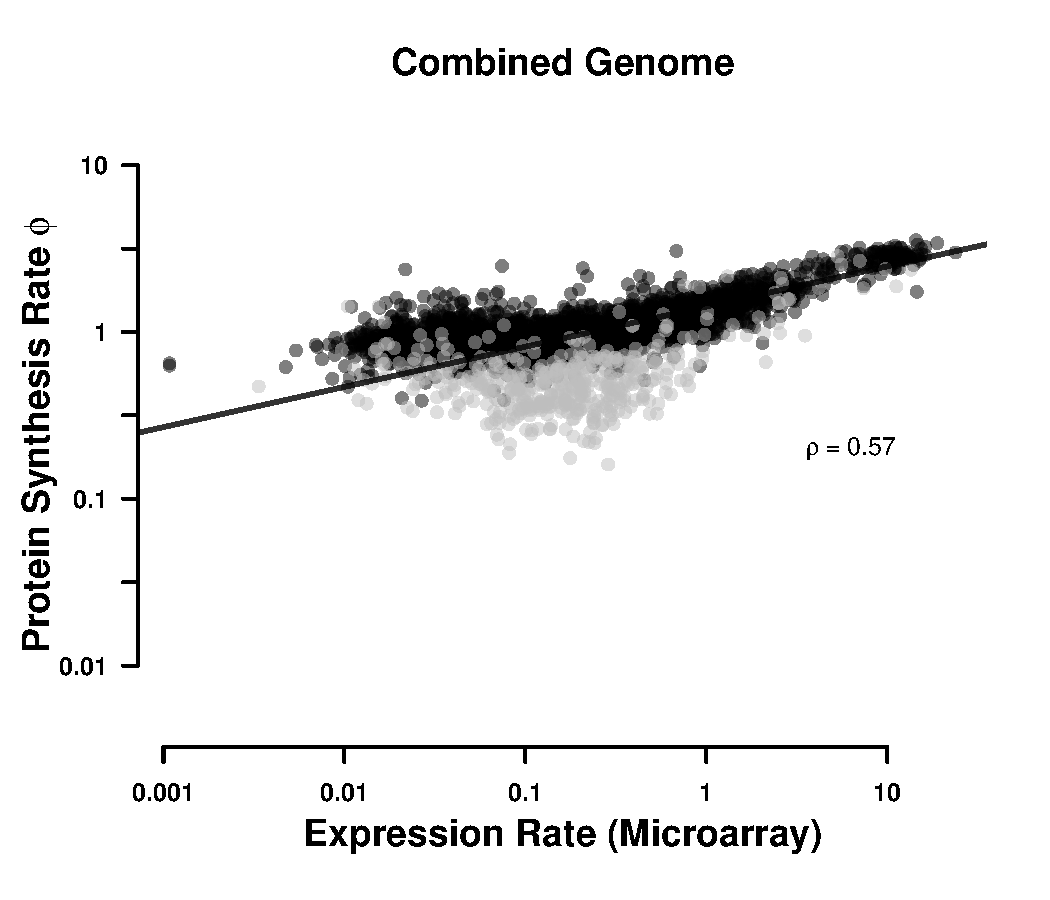
\includegraphics[width=.45\textwidth]{img/phi_corr_plot_whole_Genome_estim.pdf}
    \end{subfigure}
    \begin{subfigure}
        \centering
        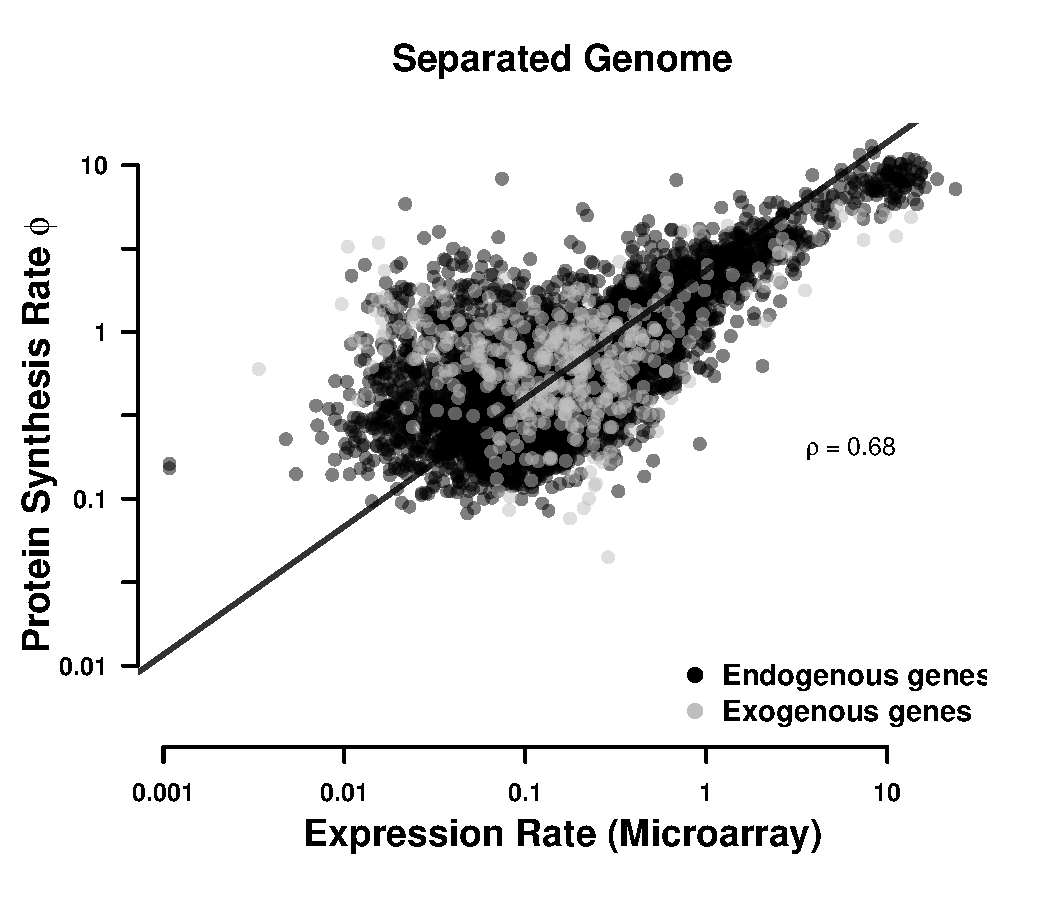
\includegraphics[width=.45\textwidth]{img/phi_corr_plot_split_Genome_estim.pdf}
    \end{subfigure}
    \caption{Person correlation of predicted protein synthesis rate $\phi$ with observed expression rate. )}
    \label{fig:phi_corr_two_cond}
\end{figure}


\begin{figure}[H]
     \centering
	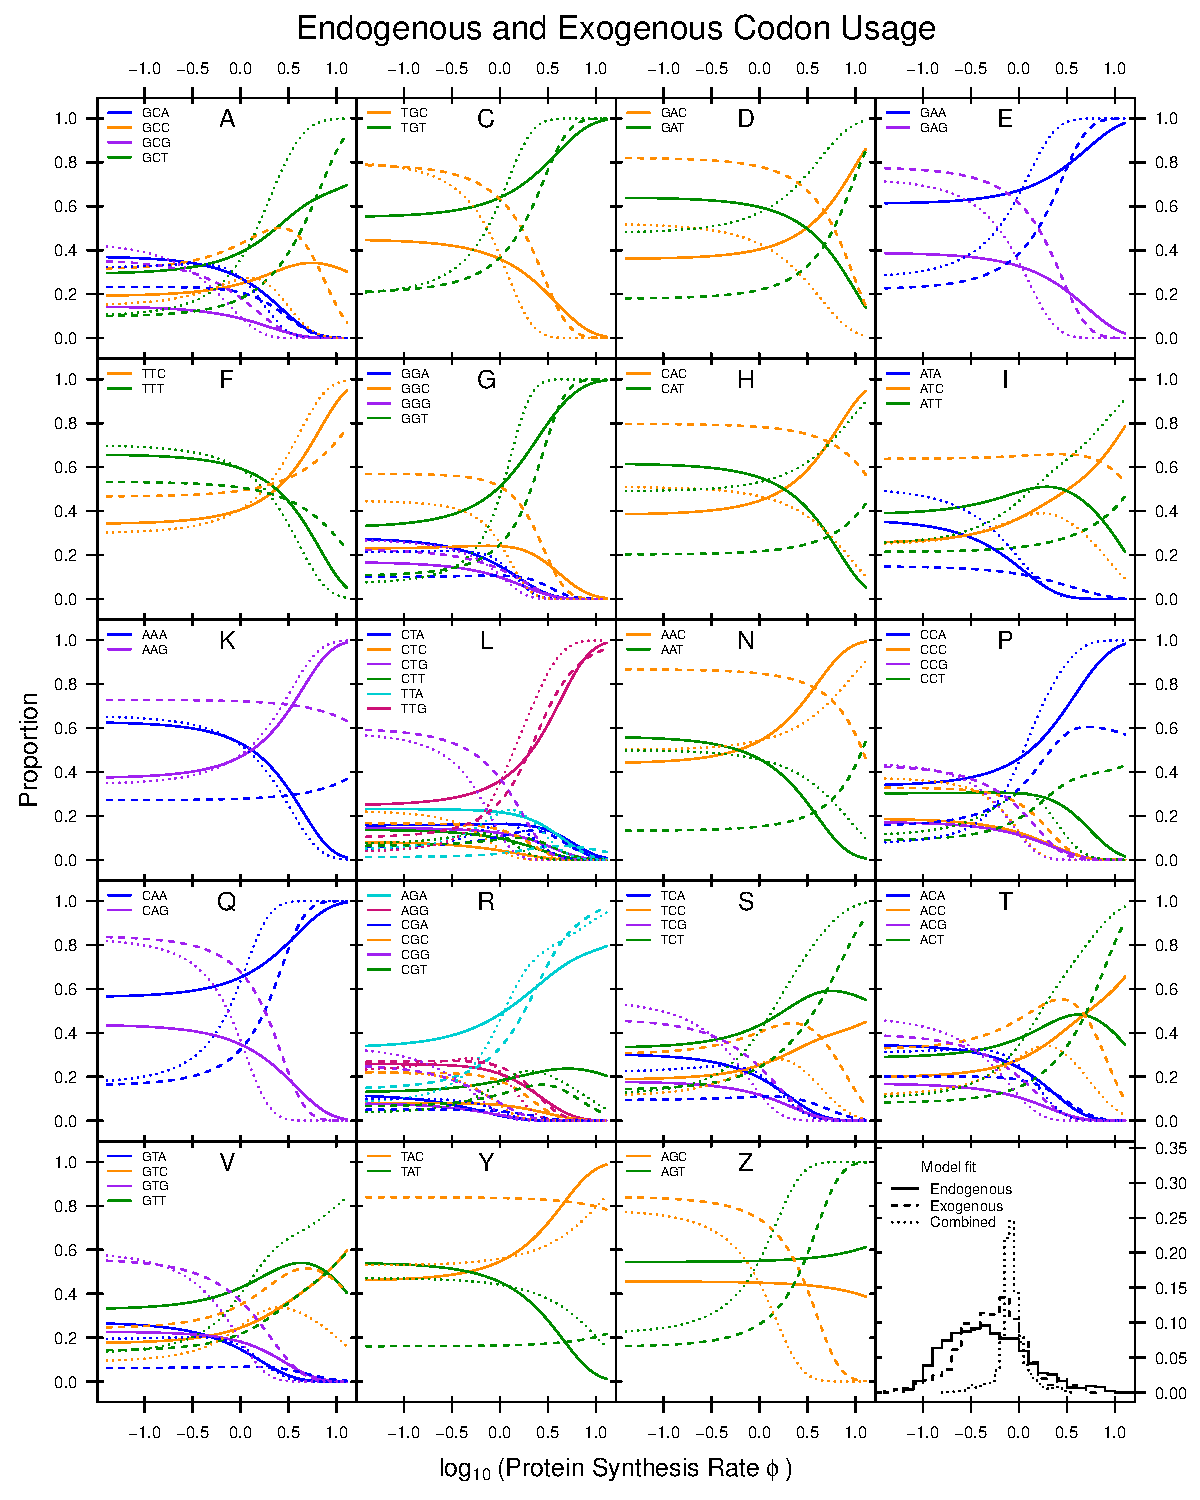
\includegraphics[width=\textwidth]{img/CUB_cleft_main.pdf}
	\caption{Codon Usage}
	\label{fig:cub_all_aa}
\end{figure}


\begin{figure}[H]
     \centering
	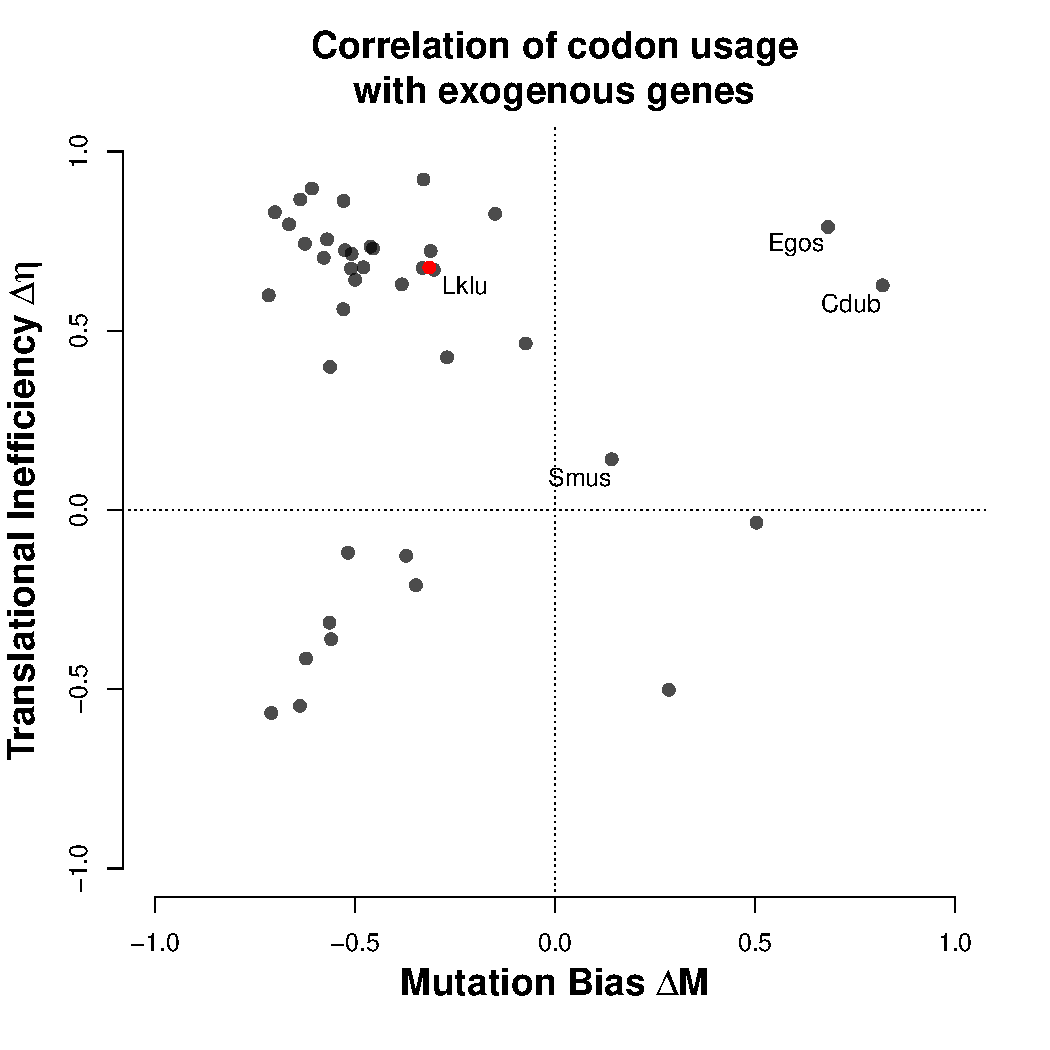
\includegraphics[width=\textwidth]{img/csp_correlations.pdf}
	\caption{Codon Usage}
	\label{fig:corr_all_species}
\end{figure}


\begin{figure}[H]
     \centering
	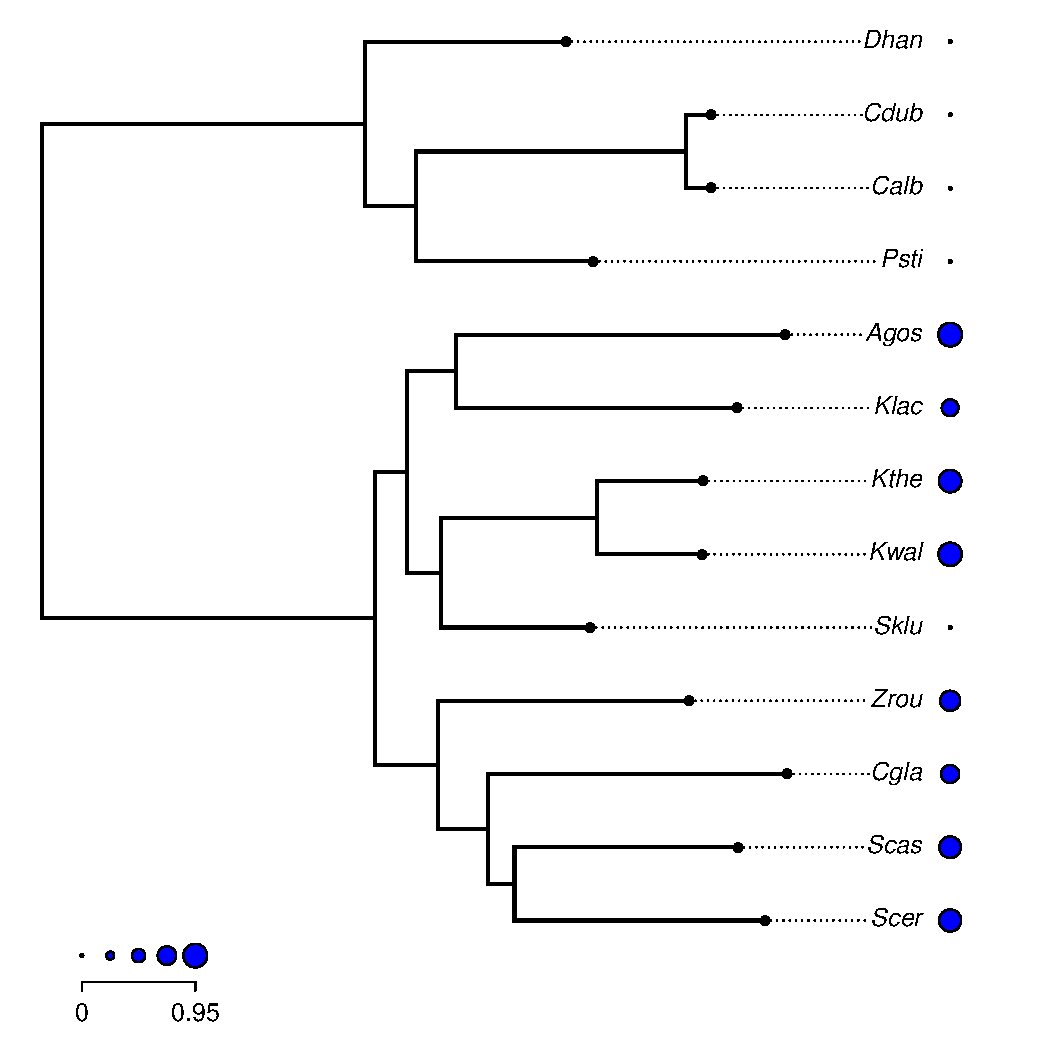
\includegraphics[width=\textwidth]{img/synteny_coverage.pdf}
	\caption{Codon Usage}
	\label{fig:synteny_species}
\end{figure}

\end{document}








